\documentclass[11pt]{article}
\usepackage[a4paper,margin=1in]{geometry}
\usepackage[T1]{fontenc}
\usepackage{textcomp}
\usepackage{amsmath,amssymb,booktabs,array,tabularx}
\usepackage{graphicx}
\usepackage[authoryear,round]{natbib}
\usepackage[hidelinks]{hyperref}
\newcolumntype{Y}{>{\raggedright\arraybackslash}X}
\title{Class Imbalance in Histopathology:\\What Separates {BRACS} from {TCGA-UT}\\Before Any Imbalance}
\author{Yannik Queisler}
\date{November 7, 2026}

\begin{document}
\raggedbottom
\widowpenalty=10000
\clubpenalty=10000
\setlength{\emergencystretch}{2em}
\maketitle
\begin{abstract}
\noindent With balanced training data, a logistic-regression readout on frozen Virchow2 features reaches 72.1\% patient-macro balanced accuracy on TCGA-UT but only 39.6\% on BRACS. This report explains, for a reader without pathology training, what the two tasks ask, what a single image patch contains, and what the frozen representation and the fitted classifier distinguish. It adds new descriptive analyses of existing features and stored predictions, with no new model fits. In the original feature space, the share of a test patch's 15 nearest training patches that carry its own class, adjusted for chance, is 0.55 on TCGA-UT and 0.20 on BRACS. The difference between datasets persists for cosine and Euclidean distance and for 5 to 30 neighbours. Classes with higher neighbour agreement are also recognised more reliably by the classifier. On BRACS, 74\% of the patch variation within a class lies within individual patients, against 52\% on TCGA-UT. The classifier's preference for the true class over its strongest rival is small for most BRACS patients: 67\% of the patient-macro mass lies within one nat of a tie, against 25\% on TCGA-UT. Under a class-prevalence ratio of 100, BRACS loses 46\% of its balanced-correct predictions, while TCGA-UT loses 10\%; both fix a similar share of their balanced errors, 17\% and 15\%. On both datasets the losses concentrate on correct predictions within one nat of a tie, but at equal margin BRACS still loses more. The neighbour comparison uses the same training support on both datasets, so the mixing is not an artefact of sample size. These observations describe where the two datasets differ. They do not identify a single cause: physical field of view, class taxonomy and label context differ between the datasets and are not varied here.
\end{abstract}

\section{Introduction}
\label{sec:intro}
Both datasets pass through the same pipeline. Each image patch is encoded once by the frozen Virchow2 foundation model \citep{zimmermann2024virchow2}, and a multinomial logistic regression is fit on the resulting 2,560-dimensional features. The headline metric is \emph{patient-macro balanced accuracy}: within each true class, patches are first averaged per patient, then patients are averaged, and the resulting per-class recalls are averaged with equal weight. A patient whose tissue carries two lesion classes contributes once to each class. With balanced training data this metric reaches 72.06\% on TCGA-UT and 39.57\% on BRACS, averaged over three patient-disjoint splits with ten training draws each \citep{queisler2026prevalenceTcga, queisler2026prevalenceBracs}. The chance level, one over the number of classes, is 3.3\% for TCGA-UT's 30 classes and 14.3\% for BRACS's seven.

These two numbers describe two experimental regimes, not an intrinsic ranking of the datasets. TCGA-UT trains on 20 patients and 640 patches per class, BRACS on 10 patients and 320 patches. One BRACS input spans about 64~\textmu m of tissue, one TCGA-UT input between 128 and 256~\textmu m. Each test split contains 1,067 TCGA-UT patients against 24 BRACS patients. Earlier studies on the same design show that class imbalance damages BRACS more than TCGA-UT \citep{queisler2026prevalenceTcga, queisler2026prevalenceBracs}. Attempts to explain that difference stopped at their pre-registered gates for different reasons. Injecting the observed prior shift into stored balanced predictions overstated the fitted damage \citep{queisler2026marginTcgaBracs}. Increasing BRACS's class separation increased rather than reduced its damage \citep{queisler2026separationTcgaBracs}. BRACS's classes fell outside TCGA-UT's range of class properties, so class composition could not be separated from dataset identity \citep{queisler2026classProperties}. A joint separation and centre-correction rescue did not survive fixed regularization \citep{queisler2026jointMechanism}. Patch reselection could not change support coverage enough to test its contribution \citep{queisler2026supportCoverage}. Better regularization selection closed less than half of the prior-only gap \citep{queisler2026lambdaSelection}. None of these outcomes refutes the proposed explanation; each leaves it untested or only partly supported. This report returns to the balanced condition. It asks what differs visibly and measurably before imbalance, then briefly examines how those differences appear under imbalance.

\section{Pathology background}
\label{sec:tissue}
Haematoxylin and eosin (H\&E) staining colours cell nuclei purple-blue and most other tissue pink. In both datasets the relevant structures are nuclei, sheets of epithelial cells that line glands and ducts, and the surrounding connective tissue, or stroma. In the breast, epithelium lines a branching system of ducts and lobules embedded in stroma and fat \citep{brancati2022bracs}.

TCGA-UT asks \emph{which cancer is this}, across 30 cancer types from many organs. Its patches were cropped by the dataset authors from tumour regions that pathologists had delineated as uniform, so most patches show cancerous tissue typical of the source slide \citep{komura2022universalEncoding}. Many classes differ by organ, and organs differ in tissue architecture; some do not. Colon and rectal adenocarcinoma, for example, arise from the same type of intestinal lining.

BRACS asks \emph{which kind of breast lesion is this}, among seven categories: normal tissue (N), pathological benign lesions (PB), usual ductal hyperplasia (UDH), flat epithelial atypia (FEA), atypical ductal hyperplasia (ADH), ductal carcinoma in situ (DCIS) and invasive carcinoma (IC) \citep{brancati2022bracs}. These categories are clinical groupings, not points on one linear disease scale: PB alone combines more than ten distinct benign entities, and UDH, ADH and DCIS all grow inside ducts. The dataset paper names one pair as especially hard. ADH has cytological atypia similar to that of low-grade DCIS but spans no more than 2~mm or only partially involves ducts; in some cases it ``includes all the features of DCIS, but is simply limited in size'' \citep{brancati2022bracs}. During annotation, pathologists sometimes had to examine the whole slide to decide between such classes \citep{brancati2022bracs}.

\begin{figure}[t]
  \centering
  \begin{minipage}[b]{0.62\textwidth}
    \centering
    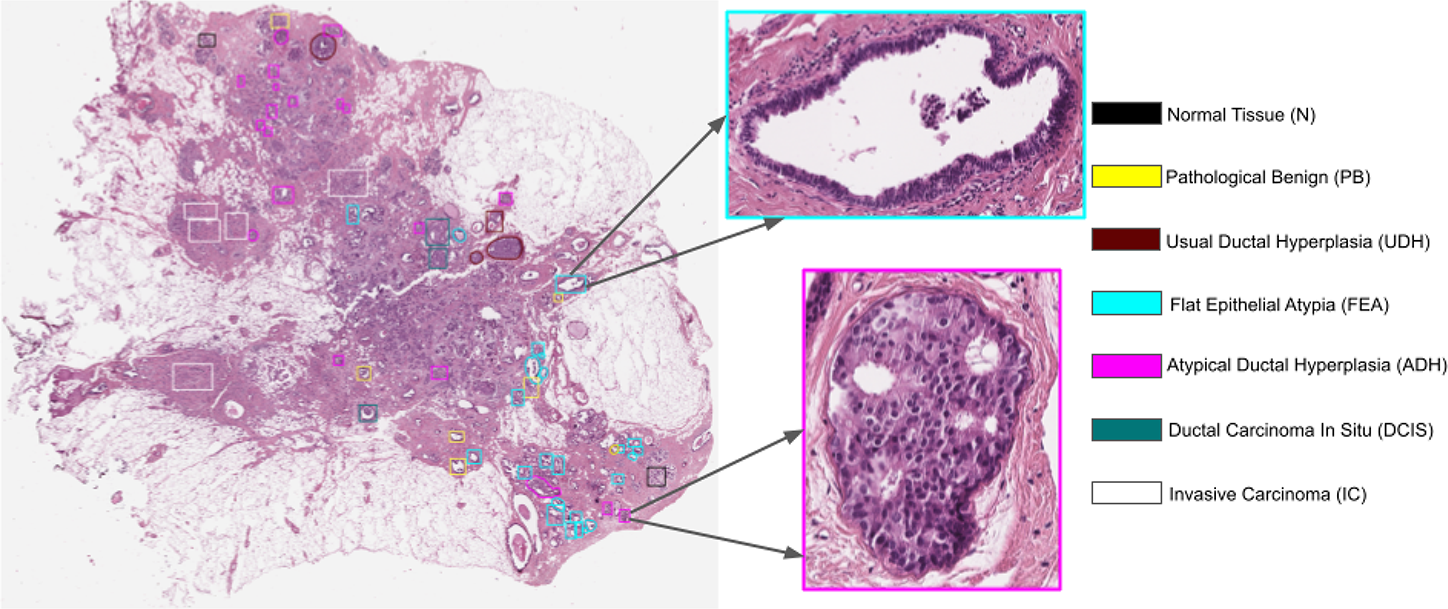
\includegraphics[width=\linewidth]{figures/brancati2022_fig1_wsi_rois.png}\\[-1pt]
    {\footnotesize (a) Slide with annotated regions of interest}
  \end{minipage}\hfill
  \begin{minipage}[b]{0.34\textwidth}
    \centering
    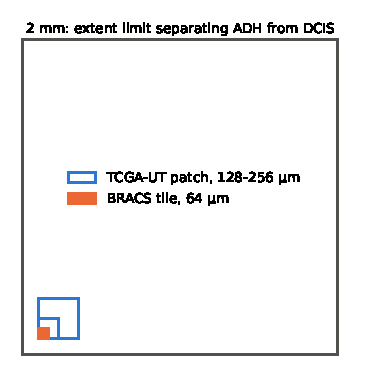
\includegraphics[width=\linewidth]{figures/scale.pdf}\\[-1pt]
    {\footnotesize (b) Field of view of one model input}
  \end{minipage}\\[8pt]
  \begin{minipage}[b]{0.40\textwidth}
    \centering
    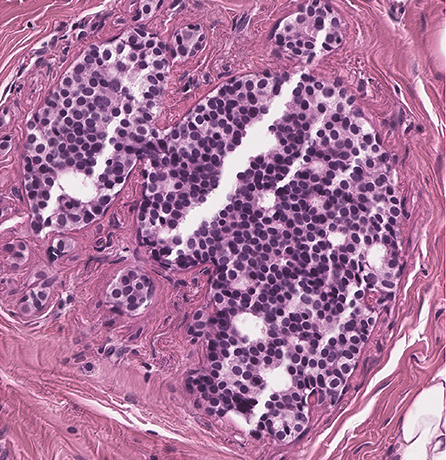
\includegraphics[height=3.9cm]{figures/brancati2022_fig3e_adh.png}\\[-1pt]
    {\footnotesize (c) ADH region}
  \end{minipage}\hspace{0.04\textwidth}
  \begin{minipage}[b]{0.52\textwidth}
    \centering
    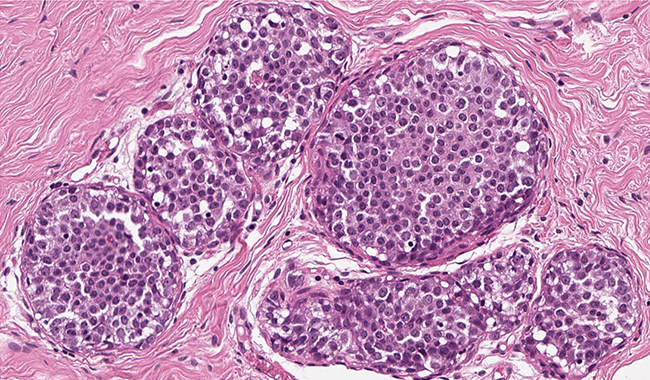
\includegraphics[height=3.9cm]{figures/brancati2022_fig3f_dcis.png}\\[-1pt]
    {\footnotesize (d) DCIS region}
  \end{minipage}
  \caption{A BRACS label belongs to a whole annotated region, while the model sees one small tile. (a) A BRACS slide with its annotated regions; colour marks the lesion class. (b) Physical extent of one model input against the 2~mm extent that separates atypical ductal hyperplasia (ADH) from ductal carcinoma in situ (DCIS), drawn to scale: a BRACS tile spans 64~\textmu m, a TCGA-UT patch 128--256~\textmu m. (c, d) Published example regions of ADH and DCIS. The dataset paper describes ADH as monomorphic cells that only partially fill the ductal spaces, and DCIS as a proliferation that fills the entire duct. Panels (a), (c) and (d) are reproduced from \citet{brancati2022bracs}, Figures~1 and~3(e, f), under CC BY-NC~4.0 (\url{https://creativecommons.org/licenses/by-nc/4.0/}); (c) and (d) are cropped, and the source gives no scale. Panel (b) is a schematic, not an image.}
  \label{fig:context}
\end{figure}

Figure~\ref{fig:context} shows why the size of an input matters. A BRACS region of interest is cut into non-overlapping $256\times256$-pixel tiles at the scanner's native 0.25~\textmu m per pixel, and every tile inherits the region's label. Each tile therefore covers $64\times64$~\textmu m, which is a few cell diameters. Virchow2's preprocessing resizes the whole tile to $224\times224$ pixels without cropping. A region of ADH can be up to 2~mm across, roughly thirty tiles in each direction, and some of its tiles show only stroma between the atypical ducts. The 2~mm extent criterion that separates ADH from DCIS cannot be seen inside any single tile. TCGA-UT patches cover two to four times more tissue in each direction, and they were selected from uniform tumour areas \citep{komura2022universalEncoding}. These differences are candidate contributors to the accuracy gap. They are not varied or measured as causes in this report.

\section{Descriptive analyses}
\label{sec:methods}
All analyses reuse stored artefacts. Predictions come from the balanced training arm (r1) and three arms at prevalence ratio $\rho=100$: the combined long-tailed arm (r100), a prior-only arm with balanced support (P100), and a support-only arm with a balanced prior (S100) \citep{queisler2026prevalenceTcga, queisler2026prevalenceBracs, queisler2026causeTcga, queisler2026causeBracs}. Each arm has three splits and ten draws, giving 30 fits per arm and dataset. The analysis maps every stored fit to one fixed class order and joins it to its test patches by manifest position. Each fit's labels must match the manifest's class names, and its recomputed patient-macro balanced accuracy must match the stored value to within $10^{-9}$. All 240 fits pass these checks. The pooled means reproduce the source studies' estimates to within $10^{-10}$ percentage points (r1: 72.06 and 39.57). Each split--draw fit receives equal weight. Results are descriptive point estimates; the analysis computes no new intervals and never treats patches as independent samples.

\paragraph{Confusion and margins.} Confusion matrices use the same patient weighting as the headline metric, so each row sums to one and the mean diagonal equals balanced accuracy. The \emph{margin} of a test patch is $\log p_{\text{true}} - \max_{d\neq\text{true}} \log p_d$, the classifier's log-probability preference for the true class over its strongest rival. A positive margin means a correct prediction. The weighted share of positive margins reproduces balanced accuracy exactly; no ties occur. Margins are also shown after dividing by each fit's stored validation temperature \citep{guo2017calibration}. Both versions are score-based summaries whose scale depends on regularization and calibration; a margin is not a distance in feature space.

\paragraph{Neighbour agreement.} For each split, the analysis draws a reference set from training patients: 10 patients per class with 32 randomly chosen patches each, so every class has equal mass. It draws a query set from the same split's test patients: up to 10 patients per class and up to 32 patches each, weighted per patient and class. The reference therefore has the same support on both datasets, 320 patches from 10 patients per class, and includes only patients with at least 32 patches in a class. Checks confirm that reference and query patients are disjoint, as required by the design. For each query patch, \emph{neighbour agreement} is the share of its $k$ nearest reference patches that carry its own class. The analysis uses the full 2,560-dimensional features, measuring cosine distance on normalised features and, separately, Euclidean distance on raw features. The main setting is $k=15$, with $k=5$ and $k=30$ as sensitivity checks. Because the datasets have different class counts $K$, the analysis also reports chance-adjusted agreement, $(a-1/K)/(1-1/K)$, where $a$ is raw neighbour agreement. This quantity is 0 at chance and 1 for perfect agreement. This adjustment does not make the two taxonomies comparable; it only removes the trivial effect of $K$. For each class in the same reference sets, the analysis also computes the share of within-class patch variance that lies within individual patients. Principal component analysis (PCA), fitted on the reference set and applied to the query set, illustrates the structure; only measurements in the original feature space support numerical statements.

\paragraph{Examples.} A fixed rule selects example tiles from the first split. For each class, it selects the query patch whose neighbour agreement is closest to the class median, together with its nearest reference patch from the confusion partner (ADH and DCIS, colon and rectal adenocarcinoma) and from any other class. The pairs follow the BRACS dataset paper and an earlier TCGA-UT study that identified colon and rectal adenocarcinoma as confusion partners \citep{brancati2022bracs, queisler2026tailTcga}. The best-recognised class serves as a counterexample. The tiles are copied unaltered from the image archives that produced the features. These post hoc selections illustrate the summaries but add no confirmatory evidence.

\section{Representation geometry}
\label{sec:geometry}
TCGA-UT test patches sit among training patches of their own class far more often than BRACS patches do. At $k=15$ with cosine distance, raw agreement is 0.56 on TCGA-UT against a chance level of 0.03, and 0.32 on BRACS against 0.14. After chance adjustment this is 0.55 against 0.20 (Figure~\ref{fig:geometry}). The difference is stable across all three splits (TCGA-UT 0.54--0.56, BRACS 0.20--0.22), across $k$ from 5 to 30, and across both distances: Euclidean distance on the raw features gives 0.55 and 0.20. The conclusion therefore does not depend on the metric, and because both reference sets have the same support, it is not a consequence of BRACS's smaller training cohort. Within TCGA-UT, classes range from 0.13 to 0.97; all seven BRACS classes fall below 0.45.

\begin{figure}[t]
  \centering
  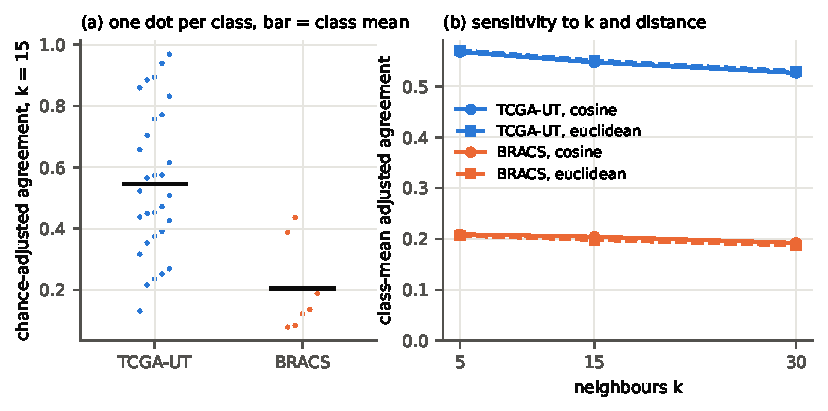
\includegraphics[width=\textwidth]{figures/geometry.pdf}
  \caption{In the original feature space, BRACS test patches have far fewer same-class neighbours among training patches than TCGA-UT patches do. (a) Chance-adjusted share of the 15 nearest training patches with the query's class, one dot per class, averaged over three splits; bars mark class means. (b) Class means for $k=5$, 15 and 30, for cosine (circles, solid) and raw Euclidean distance (squares, dashed); the two distances nearly coincide.}
  \label{fig:geometry}
\end{figure}

Classifier performance follows this geometry. Across classes, neighbour agreement and balanced-fit recall have a Spearman rank correlation of 0.96 on TCGA-UT (30 classes) and 0.82 on BRACS (7 classes). Neighbour agreement uses a fixed training sample and no classifier, so the two measures do not derive from the same predictions. Classes with mixed neighbourhoods are also harder for the readout to recognise.

Two further measurements describe how the mixing is organised. First, on BRACS 74\% of the within-class patch variance lies within individual patients, against 52\% on TCGA-UT. A BRACS patient's own tiles are thus nearly as varied as tiles from different patients, consistent with every tile inheriting the label of a heterogeneous region. Second, an earlier study reported a class-centre separation index of 0.44--0.48 on BRACS and 0.68--0.71 on TCGA-UT \citep{queisler2026separationTcgaBracs}. The index divides the median distance between nearest class centres by the pooled spread of \emph{patient means}. It measures how far apart class averages lie relative to patient-to-patient variation. Neighbour agreement measures how individual patches mix. Both indicate the same pattern but measure different quantities.

\begin{figure}[t]
  \centering
  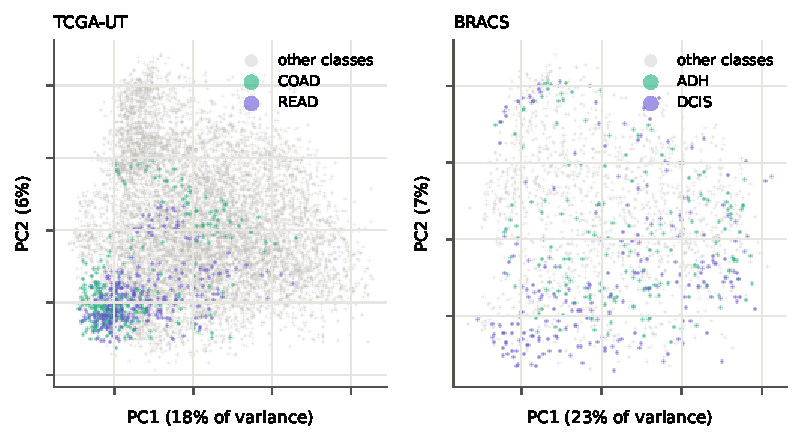
\includegraphics[width=\textwidth]{figures/pca.pdf}
  \caption{A two-dimensional projection shows the confusion pairs overlapping on both datasets. Held-out test patches from the first split are projected onto each dataset's own principal component analysis (PCA) axes, fitted on that split's balanced training sample. The highlighted classes form each dataset's confusion pair; all other classes are grey. The two panels have separate axes, so distances and cluster areas cannot be compared between panels. The first two components explain 23\% (TCGA-UT) and 30\% (BRACS) of the variance.}
  \label{fig:pca}
\end{figure}

Figure~\ref{fig:pca} shows both confusion pairs in two dimensions. Colon and rectal adenocarcinoma occupy the same corner of TCGA-UT's projection, apart from most other classes. ADH and DCIS spread across BRACS's projection among all other classes. The two components retain only a quarter to a third of the variance, so the projection illustrates the high-dimensional result but cannot replace it.

\section{Balanced decisions}
\label{sec:decisions}
On BRACS, only IC (69\% recall) and normal tissue (60\%) are recognised in most cases. ADH is recognised in 12\% of the patient-macro mass, below the seven-class chance level. It is predicted as FEA (23\%), UDH (21\%) and DCIS (18\%) more often than as itself, and DCIS in turn is predicted as ADH in 18\% (Figure~\ref{fig:decisions}a). Normal tissue and PB exchange 23\% and 32\% of their mass. On TCGA-UT, recall ranges from 28\% for oesophageal carcinoma to 95\% for thyroid carcinoma, and 21 of 30 classes exceed 65\% (full matrix in Appendix~\ref{app:confusion}). The classifier predicts colon adenocarcinoma as rectal adenocarcinoma in 36\% of the patient-macro mass, and rectal as colon in 27\%. It predicts oesophageal carcinoma as head-and-neck squamous cell carcinoma in 19\% and as stomach adenocarcinoma in 15\%. On average, a class's strongest rival takes 34\% of its errors on TCGA-UT and 35\% on BRACS. With 29 possible rivals on TCGA-UT, that is ten times the share an even spread would give; with six on BRACS, it is twice. TCGA-UT's errors thus concentrate on a few anatomically or histologically related classes, while BRACS's spread over most of the matrix.

\begin{figure}[t]
  \centering
  \begin{minipage}[b]{0.43\textwidth}
    \centering
    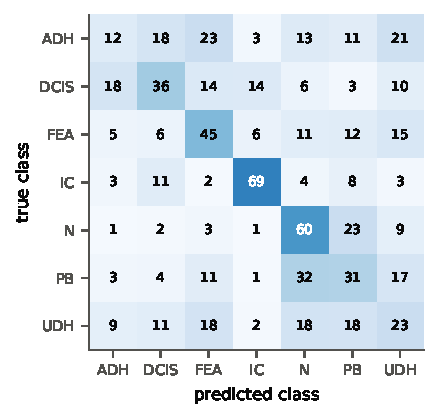
\includegraphics[width=\linewidth]{figures/confusion_bracs.pdf}\\
    {\footnotesize (a) BRACS confusion (\%)}
  \end{minipage}\hfill
  \begin{minipage}[b]{0.55\textwidth}
    \centering
    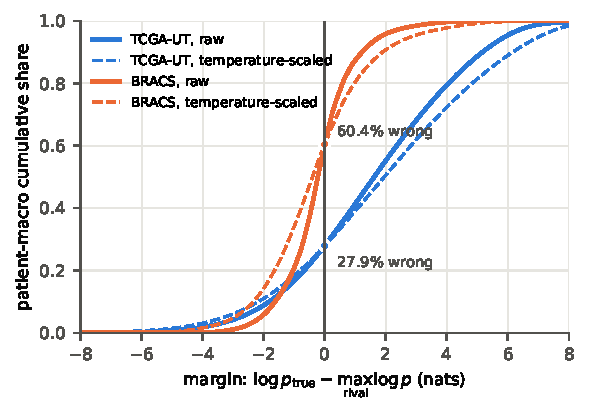
\includegraphics[width=\linewidth]{figures/margins.pdf}\\
    {\footnotesize (b) Margin distribution}
  \end{minipage}
  \caption{BRACS errors are spread over most class pairs, and most BRACS predictions are close to a tie. (a) Patient-macro confusion of the balanced fits on BRACS; each row sums to 100\% and the diagonal is per-class recall. (b) Patient-macro cumulative distribution of the true-class margin, raw (solid) and after validation temperature scaling (dashed). The value at zero is the error rate, one minus balanced accuracy.}
  \label{fig:decisions}
\end{figure}

The margin distribution shows how decisive the classifier is (Figure~\ref{fig:decisions}b). On TCGA-UT the median of the patient-macro margin distribution is 1.65 nats: the typical patient's true class is about five times more probable than its strongest rival. On BRACS the median is $-0.20$ nats, so for more than half of the patient-macro mass a rival class wins. Two thirds of BRACS's mass lies within one nat of a tie, against a quarter of TCGA-UT's. Temperature scaling stretches both distributions on average, because the mean fitted temperatures are below one (0.65 and 0.84; individual fits range from 0.30 to 1.19), but it does not change their ordering or the sign of any margin. Weighting matters here: pooling patches without patient weighting puts BRACS's median at $+0.32$ nats (averaged over fits), because each patient then counts in proportion to its number of patches. Patch-pooled margin summaries from earlier work \citep{queisler2026marginTcgaBracs} are therefore not patient-macro results.

\begin{figure}[t]
  \centering
  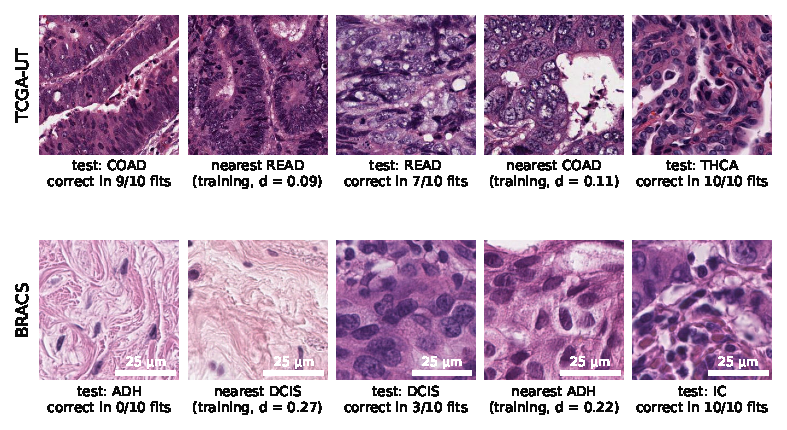
\includegraphics[width=\textwidth]{figures/tiles.pdf}
  \caption{Example test tiles and their nearest training neighbours from the confusion partner. Each test tile is the one closest to its class's median neighbour agreement; ``correct in $n$/10'' counts the balanced fits of the first split that classify it correctly, and $d$ is the cosine distance. The right column shows the best-recognised class. BRACS tiles carry a 25~\textmu m scale bar; TCGA-UT patches span 128--256~\textmu m, recorded per dataset rather than per patch, so they carry none. Selections are post hoc illustrations, not representative samples.}
  \label{fig:tiles}
\end{figure}

Figure~\ref{fig:tiles} makes these summaries concrete. The colon and rectal adenocarcinoma tiles show glandular tumour tissue of similar appearance, and each test tile's nearest partner-class tile lies at a cosine distance of only 0.09--0.11. The median-agreement ADH tile shows mainly pink stroma with few nuclei. It carries the ADH label because it was cut from an ADH region, and none of the ten balanced fits classifies it correctly. Its nearest DCIS training tile is also mostly stroma. The DCIS tile and its nearest ADH neighbour both show crowded, rounded nuclei, the shared cytology the dataset paper describes. These are single examples and do not estimate how often each pattern occurs. They show that a 64~\textmu m tile can lack the structure on which its inherited label depends.

\section{Prediction changes under imbalance}
\label{sec:imbalance}
At $\rho=100$, total damage is 7.65 points on BRACS and 2.91 on TCGA-UT; the prior-only and support-only arms isolate each channel \citep{queisler2026causeTcga, queisler2026causeBracs}. Because balanced and imbalanced fits use the same test patches, each change in balanced accuracy splits exactly into balanced-correct predictions that are lost and balanced errors that are fixed (Figure~\ref{fig:imbalance}). The net damage is much smaller than the turnover on both datasets. At r100, BRACS loses 18.1 points of correct predictions and gains 10.4; TCGA-UT loses 7.2 and gains 4.3.

\begin{figure}[t]
  \centering
  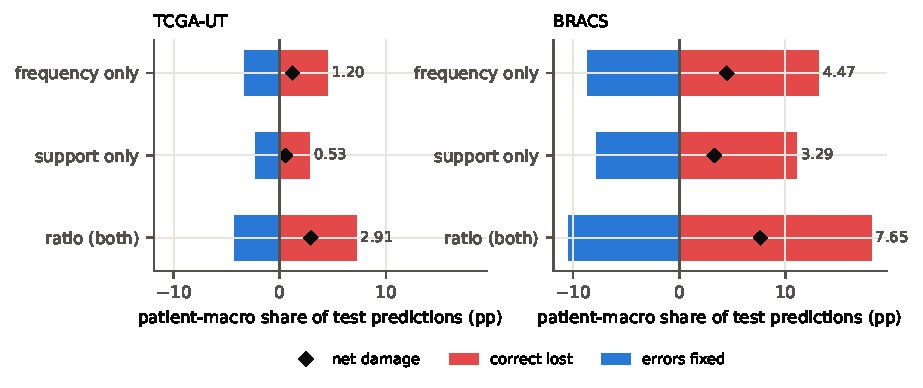
\includegraphics[width=\textwidth]{figures/imbalance.pdf}
  \caption{Imbalance moves many more BRACS predictions in both directions. For each arm at $\rho=100$, balanced-correct predictions that become wrong (red, right) and balanced errors that become correct (blue, left), in patient-macro percentage points; the diamond and number give the net damage, which equals the difference exactly.}
  \label{fig:imbalance}
\end{figure}

Relative losses of balanced-correct predictions differ more than relative gains from balanced errors. BRACS loses 46\% of its balanced-correct mass at r100, TCGA-UT 10\%. Of their balanced errors, BRACS fixes 17\% and TCGA-UT 15\%. Table~\ref{tab:margin-bins} splits the balanced-correct mass by its balanced margin. On both datasets the loss rate falls steeply with margin, from 62\% (BRACS) and 45\% (TCGA-UT) for margins up to 0.5 nats to 8\% and 2\% between 2 and 4 nats. Because 68\% of BRACS's correct mass lies within one nat of a tie, against 19\% of TCGA-UT's, that region supplies 85\% of BRACS's lost mass and 70\% of TCGA-UT's. In every margin bin, however, BRACS loses more than TCGA-UT, so the different margin distributions describe much, but not all, of the difference. The prior-only and support-only arms show the same pattern: 93\% and 91\% of BRACS's lost mass, and 86\% and 89\% of TCGA-UT's, come from within one nat. This describes which predictions move, not why.

\begin{table}[t]
  \centering
  \small
  \begin{tabular}{@{}lrrrr@{}}
    \toprule
     & \multicolumn{2}{c}{Correct mass (pp)} & \multicolumn{2}{c}{Lost at r100 (\%)} \\
    \cmidrule(lr){2-3}\cmidrule(l){4-5}
    Balanced margin (nats) & TCGA-UT & BRACS & TCGA-UT & BRACS \\
    \midrule
    0--0.5 & 6.5 & 17.4 & 45 & 62 \\
    0.5--1 & 6.9 & 9.6 & 29 & 48 \\
    1--2 & 13.9 & 8.5 & 13 & 29 \\
    2--4 & 24.2 & 3.8 & 2 & 8 \\
    $>4$ & 20.5 & 0.3 & 0 & 0 \\
    \midrule
    Total & 72.1 & 39.6 & 10 & 46 \\
    \bottomrule
  \end{tabular}
  \caption{Losses concentrate on near-tie predictions on both datasets, but BRACS loses more at every margin. Balanced-correct patient-macro mass in percentage points (pp) by its balanced margin, and the share of it lost at $\rho=100$, averaged over 30 fits per dataset.}
  \label{tab:margin-bins}
\end{table}

Small margins in the balanced model are consistent with large damage, but an earlier study showed that shifting the stored balanced probabilities by the observed prior overstates the fitted damage by a factor of three to nine \citep{queisler2026marginTcgaBracs}. Another study showed, in a pilot with one training draw per split, that artificially increasing BRACS's class separation raised its balanced validation accuracy but increased its total imbalance damage \citep{queisler2026separationTcgaBracs}. Better baseline separation therefore does not imply smaller imbalance damage. Small margins describe where most damage occurs but do not predict how much a refitted model will show.

\section{Evidence status}
\label{sec:evidence}
Table~\ref{tab:evidence} separates prior results, the new descriptive observations of this report, and the hypotheses that neither establishes. The new observations describe the balanced condition consistently. On BRACS, patches of different classes mix in the frozen feature space, and the patches of a single patient vary nearly as much as patches across patients. The balanced classifier spreads its errors across most class pairs, with most decisions near a tie. Under imbalance, losses concentrate on these near-tie correct predictions, although BRACS loses more than TCGA-UT even at equal margin. On TCGA-UT, confusion is concentrated in a few related pairs, and most decisions are clear.

\begin{table}[!htbp]
  \centering
  \small
  \begin{tabularx}{\textwidth}{@{}p{2.6cm}Y@{}}
    \toprule
    Status & Statement \\
    \midrule
    Established & Patient-macro balanced accuracy 72.06\% (TCGA-UT) vs.\ 39.57\% (BRACS); damage at $\rho=100$ of 2.91 vs.\ 7.65 points, with prior-only 1.20 vs.\ 4.47 and support-only 0.53 vs.\ 3.29 \citep{queisler2026prevalenceTcga, queisler2026prevalenceBracs, queisler2026causeTcga, queisler2026causeBracs}. Training support, class count, taxonomy and field of view differ between the regimes. \\
    Established & Prior-injection, separation, class-composition, joint-rescue, coverage and regularization explanations each stop at their gates, for different reasons and without refutation; frozen UNI2-h damage differs from Virchow2 by less than 1 point in point estimate, BRACS unresolved \citep{queisler2026marginTcgaBracs, queisler2026separationTcgaBracs, queisler2026classProperties, queisler2026jointMechanism, queisler2026supportCoverage, queisler2026lambdaSelection, queisler2026encoderTransfer}. \\
    New, descriptive & Chance-adjusted neighbour agreement 0.55 vs.\ 0.20, with the dataset difference persisting across both metrics and all tested $k$; class-level agreement tracks recall ($\rho_s$ 0.96 and 0.82). \\
    New, descriptive & Within-patient share of within-class variance 52\% vs.\ 74\%. \\
    New, descriptive & Median patient-macro margin 1.65 vs.\ $-0.20$ nats; 25\% vs.\ 67\% of mass within one nat of a tie. \\
    New, descriptive & At r100, 10\% vs.\ 46\% of balanced-correct predictions lost, 15\% vs.\ 17\% of errors fixed; loss rate falls with balanced margin on both, 70\% vs.\ 85\% of lost mass lies within one nat, and BRACS loses more at every margin. \\
    Unresolved & Whether the 64~\textmu m field of view, label inheritance from heterogeneous regions, or the finer taxonomy causes BRACS's mixing; none is varied here. The neighbour comparison matches training support, but the smaller BRACS cohort remains a candidate for the accuracy gap itself. \\
    Unresolved & Why small balanced margins translate into the observed amount of damage under refitting. \\
    \bottomrule
  \end{tabularx}
  \caption{Evidence status. Comparisons list TCGA-UT first. New observations are descriptive point estimates on the existing design and carry no causal interpretation.}
  \label{tab:evidence}
\end{table}

\paragraph{Limits.} The datasets are not matched in training support, scale, class count or taxonomy, and chance adjustment does not remove taxonomy differences. The neighbour analysis uses at most 10 patients per class and split; on BRACS this is the whole feasible test cohort for several classes, so per-class values rest on few patients. The reference includes only patients with at least 32 patches in a class, which favours patients with large annotated regions. The PCA panels have separate axes and retain a minority of the variance. The example tiles are post hoc selections and do not estimate prevalence; their visual descriptions follow the dataset paper and were not confirmed by a pathologist. All results are conditional on frozen Virchow2 features and a logistic-regression readout. Separating the candidate causes would require experiments that vary one factor at a time, such as the BRACS field of view or the number of training patients.

\bibliographystyle{plainnat}
\bibliography{references}

\appendix
\section{TCGA-UT confusion matrix}
\label{app:confusion}
Figure~\ref{fig:confusion-tcga} gives the full patient-macro confusion matrix of the balanced TCGA-UT fits. The largest off-diagonal cells link related classes: colon and rectal adenocarcinoma, lower-grade glioma (LGG) and glioblastoma (GBM), cutaneous melanoma (SKCM) and uveal melanoma (UVM), oesophageal, stomach and head-and-neck carcinoma, and the squamous-cell carcinomas of head and neck, lung and cervix.

\begin{figure}[h]
  \centering
  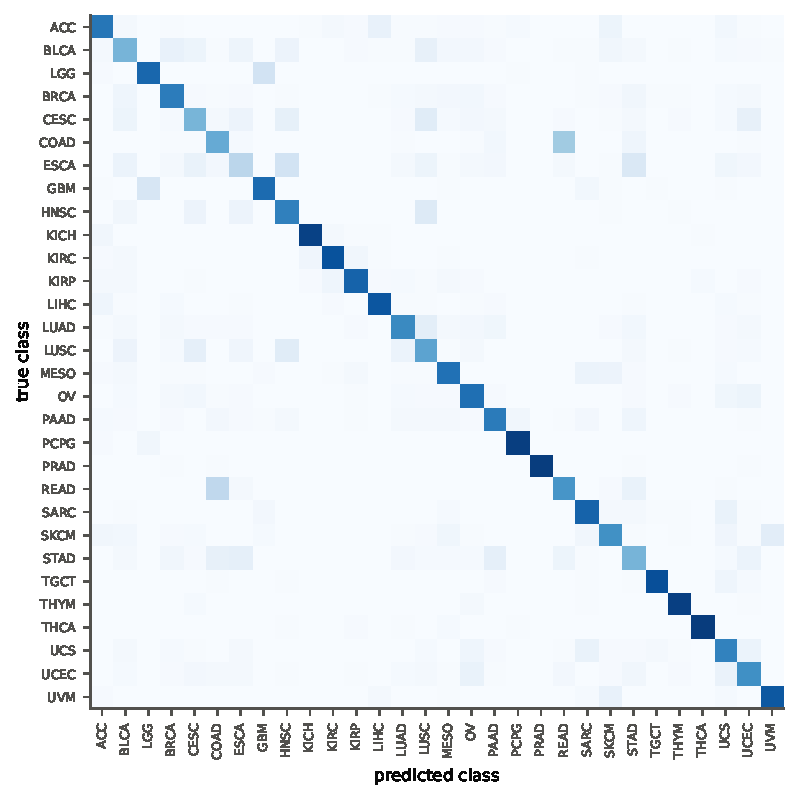
\includegraphics[width=0.92\textwidth]{figures/confusion_tcga_ut.pdf}
  \caption{Patient-macro confusion of the balanced fits on TCGA-UT (rows: true class, summing to 100\%; TCGA study abbreviations). Darker cells carry more mass.}
  \label{fig:confusion-tcga}
\end{figure}

\end{document}
